\renewcommand{\SourceFile}{5-graphes/src/5-6.ml}

\section{Ordonnancement}

Un système de tâches $(T,<<)$ est un ensemble de $n$ tâches $T=\{t_1,t_2,...,t_n\}$. Ces tâches sont liées par des contraintes de précédence : on note $t_i << t_j$ pour dire que la tâche $t_i$ doit être terminée avant que la tâche $t_j$ ne puisse commence (on dit que $t_j$ est un successeur de $t_i$, et que $t_i$ est un prédécesseur de $t_j$). Ci-dessous, on représente graphiquement un ensemble de 7 tâches, avec 8 contraintes de précédence ($t_1<<t_2$, $t_1<<t_4$, $t_2<<t_4$, $t_7<<t_2$, ...) matérialisées sous forme de flèches :
\medskip

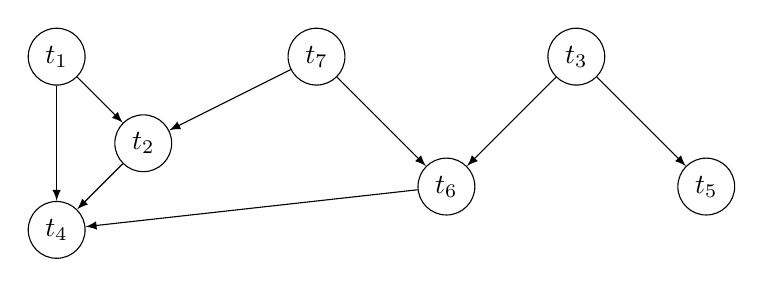
\begin{tikzpicture}[every node/.style={
    draw, circle}, -latex, scale=1.1]
    \node (1) at (0,2) {$t_1$};
    \node (2) at (1,1) {$t_2$};
    \node (3) at (6,2) {$t_3$};
    \node (4) at (0,0) {$t_4$};
    \node (5) at (7.5,.5) {$t_5$};
    \node (6) at (4.5,.5) {$t_6$};
    \node (7) at (3,2) {$t_7$};

    \draw (1) -- (2);
    \draw (1) -- (4);
    \draw (2) -- (4);
    \draw (3) -- (5);
    \draw (3) -- (6);
    \draw (6) -- (4);
    \draw (7) -- (2);
    \draw (7) -- (6);
\end{tikzpicture}
\medskip

Chaque tâche a une durée entière positive $dur(t_i)$. On dispose d'une ou plusieurs machines identiques pour exécuter les tâches. Ordonnancer le système de tâches $(T,<<)$ revient à trouver un date de début d'exécution $deb(t_i)$ pour chaque tâche $t_i$. Le but est de minimiser le temps total d'exécution tout en respectant les contraintes de dépendance : si $t_i << t_j$, on doit avoir $deb(t_i) + dur(t_i) \leq deb(t_j)$.

\Q
Proposer une structure de données pour un système de tâches et formaliser le problème. Écrire une fonction OCaml qui pour calcule pour chaque tâche le nombre et les numéros de ses successeurs et de ses prédécesseurs.

\Q
Quelle condition doivent vérifier les contraintes de précédence pour qu'il soit possible d'ordonnancer le graphe ?

\Q
On suppose la condition de la question 2 vérifiée. Pour chacun des cas suivants, proposer un algorithme pour ordonnancer le système de tâches :\\
(a) On dispose d'une seule machine ;\\
(b) On dispose de $n$ machines ;\\
(c) On dispose de $p$ machines, $1 \leq p \leq n$.

\Corrige

\Q
La structure de données la plus simple stocke les contraintes de précédence dans une matrice booléenne \texttt{c} telle que \texttt{c.(i).(j)} vaut \texttt{true} si $t_i << t_j$ et \texttt{false} sinon.
\medskip

La matrice \texttt{c} donne les successeurs. Pour trouver les prédécesseurs, il suffit de parcourir la matrice \texttt{c} et stocker les résultats dans une matrice \texttt{pred} :

\lstinputlisting[linerange={1-17}]{\SourceFile}

\Q
Il faut et il suffit que le graphe des tâches soit acyclique (sans cycle). C'est une condition nécessaire : on ne peut exécuter aucune tâche d'un cycle, et suffisante : on exécute d'abord les tâches sans prédécesseurs, puis on refait le graphe sans elles, et on recommence.

\Q
(a) Avec une seule machine, le temps total d'exécution est la somme des $n$ durées. On exécute successivement les tâches sans prédécesseurs parmi les tâches non traitées.

\lstinputlisting[firstline=19]{\SourceFile}

TODO: Finir et corriger cette section.

(b) Avec $n$ machines, il n'y a pas de problème de ressource. Par récurrence, on montre que l'optimal est d'exécuter chaque tâche au plus tôt, c'est-à-dire que la tâche $i$ est exécutée au temps $deb(j) + dur(j)$ si elle a un prédécesseur $j$ et au temps 0 sinon.
\medskip

(c) Divers algorithmes sont possibles.
\bigskip

\Fin
